%
% Simple template for generating drafts of papers and articles
%
\documentclass[12pt,]{article}
\usepackage{authblk}
\usepackage{fullpage}
\usepackage{amssymb,amsmath}
\usepackage[utf8x]{inputenc}
\usepackage[T1]{fontenc}
\usepackage{siunitx}
\usepackage{pdflscape}
\usepackage[version=3]{mhchem}
\usepackage{subcaption}
\usepackage{float}
\usepackage{tikz}

\usepackage{pdfpages}


\usepackage{natbib}
\bibliographystyle{ametsoc2014}


\usepackage[left]{lineno}
\linenumbers

\usepackage{setspace}
\doublespacing

\usepackage[unicode=true]{hyperref}
\hypersetup{breaklinks=true,
            bookmarks=true,
            colorlinks=false,
            pdfborder={0 0 0}}
\urlstyle{same} % don't use a different (monospace) font for urls

\setcounter{secnumdepth}{5}

\usepackage{todonotes}
\usepackage{graphicx}
\graphicspath{{figures/}}
% Redefine \includegraphics so that, unless explicit options are
% given, the image width will not exceed the width or the height of the page.
% Images get their normal width if they fit onto the page, but
% are scaled down if they would overflow the margins.
\makeatletter
\def\ScaleWidthIfNeeded{%
 \ifdim\Gin@nat@width>\linewidth
    \linewidth
  \else
    \Gin@nat@width
  \fihttps://www.overleaf.com/project/5d3c206cc91e240d93f4b6f6
}
\def\ScaleHeightIfNeeded{%
  \ifdim\Gin@nat@height>0.9\textheight
    0.9\textheight
  \else
    \Gin@nat@width
  \fi
}
\makeatother
\setkeys{Gin}{width=\ScaleWidthIfNeeded,height=\ScaleHeightIfNeeded,keepaspectratio}%

%%%%%%%%%%%%%%%%%%%%%%%%%%%%%%%%%%%%%%%%%%%%%%%%%%%%%%%%%%%%%%%%%%%%%%%%%%%%%%

\title{The influence of landscape features and household characteristics on risk of crop and livestock damage in the western Serengeti}
\author[1,2]{Kristen Denninger Snyder}
\author[3,4,5]{Kate Tiedeman}
\author[4,6,7]{Brendan Barrett}
\author[2,3]{Mackiana Kibwe} %is mac col state?%
\author[3]{Robert J Hijmans}
\author[2]{George Wittemeyer}

\affil[1]{Grumeti Fund}
\affil[2]{Colorado State University}
\affil[3]{Department of Environmental Science and Policy, University of California, Davis}
\affil[4]{Max Planck Institute of Animal Behavior, Department for the Ecology of Animal Societies, Konstanz, DE}
\affil[5]{Department of Computational Landscape Ecology, Helmholtz Centre for Environmental Research, Leipzig, DE}
\affil[6]{University of Konstanz, Department of Biology, Konstanz, DE}
\affil[7]{Max Planck Institute for Evolutionary Anthropology, Department of Human Behavior, Ecology, and Culture, Leipzig, DE}

%Are Brendan and I adding value other than tripling the number of affiliations?

%\affil[4]{Colorado State University}


\date{\today}

%%%%%%%%%%%%%%%%%%%%%%%%%%%%%%%%%%%%%%%%%%%%%%%%%%%%%%%%%%%%%%%%%%%%%%%%%%%%%%

\begin{document}

\maketitle
\newpage
\begin{abstract}
In rural, agriculturally dependent regions interspersed with wildlands, crop damage and livestock depredation by wildlife can threaten rural livelihoods and undermine conservation efforts. Determining the species, human activities and landscape features correlated with more or less losses to wildlife is critical to developing effective mitigation approaches. To better understand drivers of, and opportunities to reduce, wildlife damage, we surveyed 419 households in the western Serengeti of Tanzania regarding agricultural practices and wildlife-induced losses. Using a hierarchical Bayesian model, we assessed the influence of environmental and household characteristics on damage by different wildlife species. Crop loss to elephants was the most widespread form of damage, while losses to baboons and vervet monkey were less common. Landscape-level variables, particularly distance into settlements, farm visibility from the home, and presence of wooded cover, were more important than household-level variables for explaining crop damage. Livestock depredation by hyena was widespread and common, second only to crop loss by elephants in frequency. Depredation by lion was rare and localized. In contrast to correlates of crop damage, livestock depredation by lions and hyenas were driven by household-level guarding strategies. Results suggest the mitigation of livestock losses to carnivores requires localized and household-level strategies, whereas addressing crop losses to elephants requires broader, coordinated landscape-level approaches. The landscape features correlated with crop damage and livestock depredation were species specific to a greater degree than expected, indicating that species specific mitigation strategies will be more effective than generalized approaches.
\end{abstract}

\textbf{Keywords:} human-wildlife conflict, coexistence, crops, livestock, Loxodonta africana, Panthera leo, Crocuta crocuta, 

\newpage
\section{Introduction}

The ecological footprint of humans is expected to continue increasing as a result of population growth, diminishing resources and climate change \citep{Singh2010}, which is already resulting in amplified pressure on carnivores and herbivores \citep{Pimm1995, Galanti2006SpaceConservation, Woodroffe2000}. This expanding human presence, particularly along wildland edges, is restricting animal populations and increasing rates of negative human-wildlife interactions \citep{Hoare1999CoexistenceSavannas, Chen2013, Veldhuis2019}. 

Negative interactions between people and wildlife include crop damage by herbivores and livestock depredation by predators, which can negatively impact farmer livelihoods \citep{Hill2000, Kaswamila2007}, food security \citep{Hill2000, Kaswamila2007, Mackenzie2012}, and tolerance of wildlife \citep{Boer1998, Gadd2005ConservationKenya, Ogada2003, Bencin2016, Woodroffe2005, Kaltenborn2006, NaughtonTreves1997}. %Kioko et al 2006.
The links between loss of livestock to carnivores and support for lethal control and likelihood of retaliatory killing is particularly well-documented \citep{Ogada2003, Kissui2008}. The retaliatory killing of lions may be an important driver of the recent declines in lion population sizes \citep{Riggio2013, Ripple2014}. Similarly, conflict resulting from agricultural expansion into historic wildlife dominated areas is recognized to be a key driver of general wildlife declines in Africa \textbf{(Ogutu paper)}.  A primary challenge in conservation is identifying hotspots and drivers of wildlife-induced damage in order to inform and target strategies to reduce losses, thereby making such interventions more efficient. 

Determining the context and environmental drivers of wildlife-induced damage has emerged as a critical focal area for conservation. Current literature on wildlife damage often focuses on a single species or guild (e.g. carnivores), or determining the species of greatest threat in an ecosystem \citep{Dickman2013}. While critical, such an approach may under-serve the scope of the problem. In particular, few studies disentangle the environmental and human behavioral drivers of conflict with carnivorous and herbivorous species simultaneously, despite potential benefits of holistically assessing and developing mitigation plans for wildlife conflict generally in an ecosystem. Such gaps can be particularly important in mixed farming communities where households may be at risk of experiencing damage by multiple species to crops and livestock concurrently \citep{Karanth2012, Mwakatobe2014}. For instance, in East Africa, African elephants and lions have frequently been the focal species for human wildlife conflict mitigation strategies  \citep{NaughtonTreves1998,Naughton1999}, reflecting the challenges inherent in living with these two large bodied species.  However, few concomitant assessments of conflict have been conducted, despite potential benefits of leveraging actions to reduce conflict simultaneously across species. 

The drivers of damage from elephants have been notoriously difficult to disentangle \citep{Sitati2003}. While \cite{Hoare1999DeterminantsMosaic} concluded that crop damage by elephants was the result of unpredictable bull behavior, more recent studies have made significant headway in understanding the influence of environmental factors, although there is considerable variability between populations. Proximity to protected areas \citep{NaughtonTreves1998, Mackenzie2012, Guerbois2012, DenningerSnyder2019}, wooded cover \citep{NaughtonTreves1998, Nyhus2000, Graham2010PatternsConflict}, and water sources \citep{Pozo2018} are the factors most regularly associated with increases in crop damage. Elephant density and space use are not good predictors of crop damage \citep{Hoare1999DeterminantsMosaic,Pozo2018}, but seasonal fluctuations in forage quality may be an important driver in savanna ecosystems \citep{Chiyo2005}. Mixed findings of the influence of human disturbance have been reported  - studies found elephant crop damage was most likely in isolated areas \citep{Graham2010PatternsConflict,Songhurst2014}, at moderate levels of disturbance \citep{DenningerSnyder2019}, and in areas of higher human density and closer proximity to towns \citep{Sitati2003}. 

Previous work has shown that primates, particularly baboon species and vervet monkeys, frequently damage crops \citep{Mackenzie2012, Alemayehu2020, Tweheyo2005, Wallace2012}. Crop damage by primates is most likely near forest and protected area edges \citep{Hill2000,Mwakatobe2014, Saj2001, Kagoro-Rugunda2004, Wallace2012, Fehlmann2017}. In South Africa, \cite{Findlay2020} found that crop damage by chacma baboons increased in response to declining NDVI in surrounding natural habitat, but that rates of damage by vervets were not driven by changes in NDVI and instead declined in response to the presence of baboons. Primate induced crop damage has been shown to cause high cumulative losses through less severe, but more frequent raiding events; there is a need to better understand the factors influencing the risk of crop losses to primates \citep{NaughtonTreves1998}. 

Throughout East Africa, hyena and lion are the most commonly reported predator of livestock \citep{Ogada2003, Patterson2004, Mkonyi2017, Kolowski2006, Koziarski2016}. In Tanzania, hyena pose the greatest risk to livestock owned by pastoral households \citep{Kissui2019, Holmern2007}, but losses to lions have greater economic impacts and are less tolerated \citep{Muriuki2017, Kissui2019, Kolowski2006, Lichtenfeld2015}. While the seasonal timing of livestock depredation varies geographically between wet \citep{Patterson2004, Kissui2019, Kolowski2006, Mponzi2014} and dry \citep{Butler2000, Ikanda2005} periods, peaks tend to correspond with low densities of natural prey \citep{Patterson2004, Kolowski2006}. Livestock depredation is more common near water sources \citep{Abade2014,Beattie2020, Weise2019}, and risk may also be higher near tree or bush cover, but is likely to vary by species \citep{Abade2014}. Depredation by hyena is reported far from protected areas \citep{Holmern2007}, whereas depredation by lion is more often associated with close proximity to protected areas \citep{Loveridge2010,Mbise2018, Holmern2007} and low human density \citep{Weise2019}. 

Agricultural practices also influence the risk of damage by wildlife. Farm size, number of crops grown, and number of months fields are planted have been shown to influence the risk of crop loss \citep{Sitati2003, Graham2010PatternsConflict, Karanth2012,  Karanth2013,Sitati2005FactorsConflict}, %Nyirenda et al 2012, 
\todo{Should this ref be merged or did a sentence get removed}
\textbf{\citep{Sitati2005FactorsConflict}}. The use of deterrents and preventative measures, particularly those that provide advanced warning such as guarding \citep{Sitati2005FactorsConflict}, are also known to influence the risk of crop damage (for a review of deterrents, see \cite{DenningerSnyder2020}). Similarly, livestock husbandry methods influence the risk of depredation \citep{Woodroffe2005,Inskip2009}, with guarding livestock during the day and corralling at night recognized to reduce the risk of losses to predators \citep{Ogada2003}%(\textbf{Woodroffe2007})
; guarding effort \citep{Mkonyi2017} and type of enclosure \citep{Kissui2019, Lichtenfeld2015, Weise2018} further influence risk. Grazing practices that increase the encounter frequency between livestock and predators, such as seasonal grazing within protected areas, can increase depredation risk \citep{Valeix2012, Kuiper2015}.

Understanding the relative influence of household and environmental variables on the risk of wildlife-induced damage is needed in order to determine at what scale mitigation strategies should be implemented (household, community, or landscape). The economic, labor, and opportunity costs of mitigation efforts are often high  - determining the scale at which strategies will be most efficacious, in combination with consideration of factors related to local attitudes, sustainability, and scalability, can contribute to the design of an effective mitigation toolkit \citep{DenningerSnyder2020}. Relatedly, it is important to consider whether generalized strategies can be efficiently applied, or if species-specific tools are required. 

Here we examine how an integrated multi-species assessment of damage can inform prioritization and the selection of risk mitigation strategies. We evaluate the relative importance of landscape- and household-level drivers of conflict for five of the most commonly reported species causing damage: African elephant \textit{(Loxodonta africana)}, olive baboon (\textit{Papio anubis}), vervet monkey (\textit{Chlorocebus pygerythrus}), spotted hyena (\textit{Crocuta crocuta}), and lion (\textit{Panthera leo}). We model the probability of crop damage and livestock kills to identify the landscape and household characteristics driving risk. We map predictions of conflict probability across the landscape, assess how the spatial distribution of conflict drivers vary by species, and explore how such information can be utilized to identify opportunities for and challenges to human-wildlife co-existence.


%and Kushnir et al 2014 paper: 
%https://onlinelibrary.wiley.com/doi/pdf/10.1111/aje.12157

%https://environmentalevidencejournal.biomedcentral.com/articles/10.1186/s13750-019-0153-7

%https://link.springer.com/article/10.1007/s10764-018-0027-9
%https://books.google.de/books?hl=en&lr=&id=6vNzRzcjntAC&oi=fnd&pg=PA252&dq=compare+human+wildlife+conflict+animal&ots=j5gQyITw4a&sig=em0EkV3V5i4pZe_YbIzXp59GSu0#v=onepage&q=compare%20human%20wildlife%20conflict%20animal&f=false

\section{Methods}
\subsection{Study Area}

The study area is located in northern Tanzania (1$^{\circ}$45’ – 2$^{\circ}$10’ S, 33$^{\circ}$50’ – 34$^{\circ}$ 50’ E) and is comprised of communities adjacent to the Ikorongo and Grumeti Game Reserves and Ikona Wildlife Management Area (IGGR)~(Figure \ref{fig:FigGrumContext}). These protected areas form an important buffer zone between Serengeti National Park and settlements, and contain several threatened species, including cheetah (\textit{Acinonyx jubatus}), elephant (\textit{Loxodonta africana}), leopard (\textit{Panthera pardus}), lion (\textit{Panthera leo}), and black rhino (\textit{D. bicornis michaeli}) and maintains habitat critical to the seasonal migration of wildebeest (\textit{C. taurinus mearnsi}), zebra (\textit{Equus quagga}), and gazelle (\textit{Eudorcas thomsoni}) through the Greater Serengeti-Mara Ecosystem (GSME). The elephant population in IGGR totals more than 1500 animals during the dry season and has increased by an average of 7.5\% per year since 2002 \citep{Goodman2018}. The hyena population is stable, with annual estimates ranging between 400-500 individuals \citep{Goodman2018}. While the lion population size is unknown, observations indicate the species was rare in 2003 and common as of 2018 \citep{Goodman2018}. Olive baboons and vervet monkeys are locally abundant; population estimates are unavailable.

\begin{figure}
    \centering
    \includegraphics[width=\textwidth]{Figures/Area.png} %width=13 from previous paper
    \caption{Map of the western corridor of the Serengeti Ecosystem, which contains the Ikorongo and Grumeti Game Reserves, Ikona Wildlife Management Area, Serengeti National Park, and various village managed limited use areas, such as designated grazing land where permanent settlements are not allowed.}
    \label{fig:FigGrumContext}
\end{figure}

%https://blog.revolutionanalytics.com/2009/01/10-tips-for-making-your-r-graphics-look-their-best.html

This area of the GSME is characterized by a bimodal rainfall regime and one distinct dry season. Crop damage peaks during periods of ripening and harvest, typically between May and July and November and December \citep{DenningerSnyder2019}. Livestock losses are most common during the rainy seasons, peaking between March and May (Fig S1). 

Elephant-induced crop damage is commonly reported and increasing in prevalence \citep{DenningerSnyder2019}. Community members reported that wildlife-induced damage, particularly due to elephants, has the greatest detrimental impact on household security (Grumeti Fund, 2016). In Tanzania, primates are excluded from the system of consolation payments, an important source of historical data on wildlife-induced damage (Dangerous Animals Consolation Regulations of 2011); little is known locally about the influence of primates on crop loss. 

Information regarding the severity of and trends in livestock losses to carnivores is limited, but monitoring records of 284 self-reported and verified livestock losses (SI Table 1) illustrate that predators killed 1,137 livestock and injured an additional 182 in villages adjacent to IGGR between January 2017 and June 2020 (SI Table 2). Multiple retaliatory poisoning events have resulted in lion fatalities \citep{Jacob2014, Tengo2018}.

\subsection{Data Collection}
We conducted a household survey to collect data on wildlife damage characteristics in communities within 12 km of the reserve. Systematic sampling was used to cover the entire study area. We created a sampling grid composed of 3 km$^2$ cells and sampled one household per grid cell. This cell size was used to balance sampling effort and to ensure that multiple households were contained within a single cell in rural areas to protect respondents' privacy. We excluded grid cells that were inaccessible and did not contain settlements. We used high-resolution satellite images to identify uninhabited cells before sampling; additional cells were considered uninhabited when no homes could be located while surveying. In total, 419 cells were sampled (Figure~\ref{fig:sampling_schema}).

\begin{figure}
    \centering
    \includegraphics[width=\textwidth]{Figures/sampling_survey.png} %width=13 from previous paper
    \caption{Sampling frame used for the survey. 419 households were sampled (one per grid cell). Uninhabited and inaccessible cells have hash marks. All sampled households are within 12 km of the reserve.}
    \label{fig:sampling_schema}
\end{figure}

Surveys were conducted between February and July 2017 by local trained enumerators speaking Kiswahili. Questions were asked to the male or female head of household (or in their absence, another adult of 18 years or older), at the respondent’s home. Survey protocols and verbal consent documents were reviewed and approved by Ethical and Independent Review Services (protocol 17013-01).

We asked respondents questions about types of damage, species involved, agricultural practices, and household characteristics (SI). %\textbf{change to Supplementary info}.
In order to maximize the accuracy of recall and self-reporting, we asked respondents to limit responses to the previous calendar year (2016). We only evaluated losses due to mammals; respondents were provided with photos and names of wildlife species to aid accurate identification. We considered crop damage from the previous year as a binary answer. We considered livestock damage with reference to cattle, dogs, donkeys, goats, and sheep. We asked respondents to indicate how often they reported damage to local authorities for species that are listed under the Dangerous Animals Consolations Regulations \citep{URT2011} in order to evaluate reporting rates. 
 
\subsection{Environmental data}
Environmental variables were selected based on previous work indicating their relevance to crop or livestock damage (Table \ref{tab:predictorvariables}). Specifically, we considered variables related to human disturbance, habitat features, and respondents' household characteristics. 

Spatial data was derived at 30 m resolution. For variables considering the density or proportion cover of features, the environment of household locations was characterized by computing values for a surrounding buffer. We used species-specific buffer distances derived from calculated metrics of mean daily net displacement (Table~\ref{tab:radii}). To derive this metric we used GPS collar data to calculate the maximum net displacement within each defined period, averaged across all days and individuals. For carnivores, we considered overnight net displacement (17:00 - 07:00), for primates daytime net displacement (05:30 - 20:00), and for elephants 24-hr net displacement. Additional details on how variables were derived can be found in the Supporting Information.


\begin{table}[]
\centering
\footnotesize
\caption{Source of movement data for mean daily net displacement used to create species-specific radii}
%\begin{tabular}{llll}
\begin{tabular}{p{2cm}p{2cm}p{3cm}p{8cm}}
\hline
Species  & Radius & Location                          & Source                                                                                                                                                                                                 \\ \hline
Baboon   & 2.4 km  & Mpala, Kenya                      & \begin{tabular}[c]{@{}l@{}}Crofoot M. Papio Anubis (olive baboon).\\ Movebank ID: 7023252\\ Isbell LA, Bidner L. Leopards, baboons \\ and vervets in Laikipia, Kenya. \\Movebank ID: 17629305\end{tabular} \\ 
Elephants & 5 km    & western Serengeti, Tanzania       & \begin{tabular}[c]{@{}l@{}}Denninger Snyder K, Mbise N, Mjingo EE. \\ Unpublished data, 2018-2020.\end{tabular}                                                                                        \\
Hyena    & 4.3 km  & Maasai Mara, Kenya                & \begin{tabular}[c]{@{}l@{}}Holekamp K, Gersick A, Strandburg-Peshkin A,\\ Jensen F, Johnson M. Hyena communication \\and coordination – pilot. \\ Movebank ID: 914907848\end{tabular}                   \\
Lion     & 2.1 km  & Serengeti National Park, Tanzania & Craig Packer, pers. comm                                        \\
Vervet  & 500 m  & Maasai Mara, Kenya
\begin{tabular}[c]{@{}l@{}} Isbell LA, Bidner L. Leopards, baboons \\ and vervets in Laikipia, Kenya. \\Movebank ID: 17629305\end{tabular}

\\ \hline
\end{tabular}

\label{tab:radii}
\end{table}


\begin{landscape}
\begin{table}[]
\centering
\footnotesize
\caption{Predictor variables used in the study with data source and evidence of variable importance for crop and livestock damage}
\begin{tabular}{p{3cm}p{5cm}p{5cm}p{5cm}}
\hline
\textbf{Category}                       & \textbf{Predictor variable}  & \textbf{Data source}            & \textbf{Evidence of effect on conflict risk}         \\ \hline
Human presence                          & Building Density                 & Open Street Map digitized buildings       & Reduced (Sitati 2003) or increased (Songhurst 2013) risk with increasing density                  \\
                               & Distance to settlement leading edge     & Manually digitized                              & Increased risk closer to boundaries of protected areas (Schiess-Meier 2007, Butler 2000, Van Bommel 2007)         \\
                                  & Road Density      &    Grumeti Fund, OSM     & Species specific utilization or avoidance of road features                 \\
Environmental Features                                & Density of forest cover        & Landcover map (Landsat 8 Random forest)   & Increased or decreased risk at higher densities (Abade et al. 2014)      \\
                                   & Density of woodland        &  Landcover map (Landsat 8 Random forest)              & Suitable elephant habitat    \\
                         & Cropland density &  Landcover map (Landsat 8 Random forest)  & Increased risk with greater density; \\
                                    & Density of rivers        &  Serengeti GIS and Data Center              & Increased risk (lion predation) (Hopcraft 2005)  \\
                                    & Slope                    & USGS SRTM            & Decreased risk with increased slopes/visibility  \\
Household Characteristics & Farm / herd size    & Survey                 & Increased risk with increasing  farm and herd size                      \\
        & Household size    & Survey  & Decreased risk with increasing household size                      \\
                                          & Farm visibility     &     Survey              & Increased risk if unable to see farm        \\
                                  & Guarding strategies & Survey                   & Reduced risk with increased proportional guarding effort       \\       \hline                                                                           
\end{tabular}

\label{tab:predictorvariables}
\end{table}
\end{landscape}


\subsection{Causal Inference and Directed Acyclical Graphs}
A primary aim of the scientific enterprise is to infer causal effects of predictors on outcome variables of inference, so we can understand how systems function. This also can help folks working in applied contexts make informed interventions, such as mitigating human-wildlife conflict. Well-designed experiments are one typical approach to understand causality, but in many cases, like the study presented in this paper, experiments would be infeasible or unethical. Many common approaches in statistical inference, such as multivariate regression, do not make any claims about causality, and statistical information flows directly between outcome variable and predictors. Researchers are often concerned about the effect of predictor, X, on an outcome variable, Y.  However, X may be correlated with another covariate(s) of interest, Z, which can confound the relationship between X and Y. To infer the relationship between X and Y, researchers will often add covariates like Z (and often times many others) to control for potential covariates. A common term in ecology papers is to ''control for seasonality'' or ''control for environmental effects.''

Confounding factors are a real, and valid concern, but whether or not to include a variable in a multivariate regression depends on the causal relationships between measureable variables of interest, and any potential unobserved variables. In some cases, including  covariate Z can reduce the precision of an estimate of the effect of X on Y or render it entirely unreliable if Z is a collider (where X and Y both cause Z).

Directed acyclical graphs (DAGs) are a simple tool to draw out the causal relationships different components in a system (CITE Judea Perl). While common in fields such as epidemiology, they have been slower to be utlized in ecology and conservation biology \citep{Laubach_etal_CI_2021}, and have only recently been incorporated into statistical pedagogy \citep{McElreath2020}. DAGs force researchers to use their expert knowledge of their study system to draw out causal relationships between predictors and outcomes of interest. Assuming our DAG is true, DAGs can tell us if we should include a covariate in a regression as it is a confound to improve estimation of the effect of X on Y, or if should exclude it because it invalidates estimation and is misleading (collider bias). DAGs can also tell us if we need to collect information on other variables to make accurate inference, or is a question is even answerable at all to to unmeasured or unobservable confounds.

We do not go into detail and Causal Inference and DAGs, but instead direct researchers to  books \citep{pearl2009causality,McElreath2020}, papers \citep{cinelli2020crash,Laubach_etal_CI_2021} and resources \citep{textor2016robust} we have found informative for understanding DAGs . Below we draw DAGs out for our two questions of interest: What household and landscape level variables influence human-wildlife conflict for a. crop-raiding and b. livestock-raiding species.

\subsubsection{DAG for Livestock Conflict}

Things are about to get weird, and this is mostly for Kristin and Kate. We have to refine our DAGs to represent our hypotheses, and then trace the causal pathways, to see what we should include/exclude from a model to make inference. Three things jump out from our current DAG based of of Kristins drawing-- 1) We are unsure if building density directly affects the number of livestock head and 2) We are unsure if roads cause livestock-conflict. Thirdly, we have drawn a DAG that shows number of guards influences, and is influenced by livestock conflict. 
This is because the timescales are mixed up. If we draw an arrow from guards to conflict, that would imply that we collected the data on guards, before we measured the effect on conflict. I.e. we exposed guards to livestock before we measured conflict. 

This is the problem of the intervention data we currently have. We surveyed people about the prevention methods they used, and whether or not they experienced conflict. we did not measure conflict after we treated the population with guards, thus it is possible folks added more guards after they experienced conflict, to minimize it. We need a time series of data and changes in interventions (ideally more detailed than presence absence)  to get at this. Then we can draw a different causal model, and figure out analysis.

Below is link to our old DAG, we can use the maximally inclusive one. Here is url \url{http://dagitty.net/dags.html?id=ZG_AQM}


We can also do a simple one where we erase the question mark paths which seems to be what Kristin was saying, which makes some things simpler. 
% This code uses the tikz package

\begin{figure}[!h]
\centering
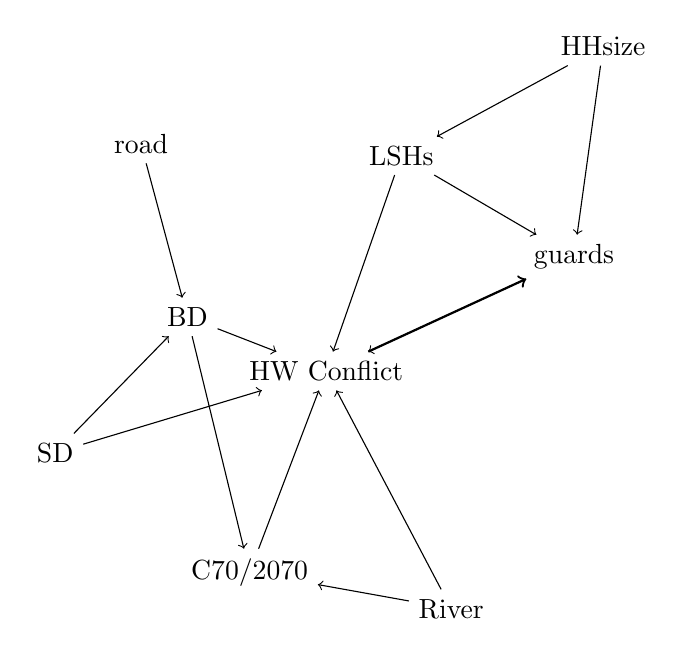
\begin{tikzpicture}
\node (v0) at (-1.04,-3.15) {C70/2070};
\node (v1) at (-0.0670,-0.593) {HW Conflict};
\node (v2) at (-1.83,0.0930) {BD};
\node (v3) at (3.45,3.53) {HHsize};
\node (v4) at (0.887,2.14) {LSHs};
\node (v5) at (1.52,-3.61) {River};
\node (v6) at (-3.51,-1.63) {SD};
\node (v7) at (3.08,0.857) {guards};
\node (v8) at (-2.42,2.29) {road};
\draw [->] (v0) edge (v1);
%\draw [->,<-] (v1) edge (v7);
\draw [thick,black,->] (v1) edge (v7);
\draw [<-] (v1) edge (v7);
\draw [->] (v2) edge (v0);
\draw [->] (v2) edge (v1);
\draw [->] (v3) edge (v4);
\draw [->] (v3) edge (v7);
\draw [->] (v4) edge (v1);
\draw [->] (v4) edge (v7);
\draw [->] (v5) edge (v0);
\draw [->] (v5) edge (v1);
\draw [->] (v6) edge (v1);
\draw [->] (v6) edge (v2);
\draw [->] (v8) edge (v2);
\end{tikzpicture}
\end{figure}

Here our target is seeing how several factors of interest might drive human wildlife-conflict over livestock. The number of livestock
We can trace the paths in it to see what we want to use, or exclude in a model to estimate any particular effect size, or we can interact with it on daggity.com and change what our outcome and predictor is.

\subsection{Modeling wildlife damage}

We created a number of hierarchical generalized linear mixed effects models. Using a Bernouli outcome with a logit link, we asked if a household experienced conflict (1) or not (0) in 2016. We had two families of models that examined the drivers of loss to the most commonly reported species. The first family was used to examine whether or not crop loss occurred due to conflict with three species: baboons, elephants, and vervets. The second family was used to examine if livestock loss occurred due to conflict with two species: hyenas and lions. In each model we estimated varying intercepts for each village. We estimated varying intercepts and slope for each species for all predictors. We estimated which model, or suite of models, best predict the data without over-fitting using Widely Applicable Information Criteria (WAIC). In the event that a single model did not take all WAIC weight, we model averaged predictions. The models were fit using the ``map2stan'' function in the R package "rethinking" \citep{McElreath2020a} which fits statistical models using Stan, a Hamiltonian Markov Chain Monte Carlo Probability sampler (Stan Development Team 2020). All code for model fitting, graphs, and raw data can be found in the supplemental material. %(repository DOI). 
All non-binary predictor variables were standardized before analysis, and effect sizes correspond to standardized data. Number of livestock head was log transformed. Model predictions on graphs are transformed back to the real (or logarithmic) scale for ease of interpretation.

We model-averaged predictions using WAIC scores to produce spatial predictions of crop damage by baboons, elephants, and vervets and livestock depredation by lions and hyenas. Landcover variables were used at a 30 m resolution and household variables were held to their standardized average (zero) to predict risk for an 'average household'. Binary ``dummy varibles'' such as ``see field'' were set to the population average for model predictions.


We checked the predictor variables for evidence of multicollinearity and found little reason for concern (Figures~S\ref{fig:pairsplotcrop},S\ref{fig:pairsplotlivestock}). The most extreme correlation was between between Cover 20/70 and crop density (-0.67) in the crop conflict data set. Parameter values in models excluding one of these two predictors did not drastically change parameter estimates. Multicollinearity is generally only a concern for interpreting individual parameter estimates of covariates; it does not affect model predictions \citep{McElreath2020}.

\section{Results}

\subsection{Survey Respondents Characteristics}

Respondents were 39 years old on average (range 18-88 years), and 50.6\% were female and 49.4\% male. Most of those surveyed (79.5\%) were born in either Bunda or Serengeti Districts. The average household size was eight people (range 2 – 28). Nearly everyone surveyed grew crops (99\%) and raised livestock (74\%). 

On average, total farm size was 2.4 hectares (range: 0.4-28), respondents grew 3 different crops (range: 1-10), and fields were planted an average of 9 months of the year (range: 2-12). Respondents typically employed multiple strategies to prevent or deter wildlife from damaging crops (mean = 2, range = 1-4), the most common being: shouting (72\%), guarding (67\%), chasing (23\%), and fire (22\%). The majority (60\%) of respondents indicated that damage due to wildlife, rather than disease, weather, depleted soils, or labor, was the greatest threat to crop production, and 98\% of those who experienced loss indicated that among wildlife species, elephants posed the greatest threat. 81\% of farming households suffered crop losses to wildlife in 2016, with elephants being the most commonly identified species (Table~\ref{tab:table1reportingrates}).  


\begin{landscape}
\begin{table}[]
\centering
\footnotesize 
\caption{Crop damage characteristics resulting from a systematic survey of households within 12 km of IGGR and Serengeti National Park. Reporting rates of buffalo damage not included because of low number of occurrences. The elephant crop damage reporting rate is estimated based on the interval responses of how likely a household was to report damage to local authorities for consolation payments.}
\begin{tabular}{lll}
\hline
\textbf{Characteristics}                      & \textbf{Details}      & \textbf{Responses} \\ \hline
Farming households                            & Total                 & 413 (99\%)         \\
Crop damage households (\%)                   & Of farming households & 81\%               \\
Households impacted by species                & Elephant              & 79\%               \\
                                              & Vervet                & 10\%               \\
                                              & Baboon                & 9\%                \\
                                              & Bushpig               & 2\%                \\
                                              & Hippopotamus          & 1\%                \\
                                              & Buffalo               & \textless 1\%      \\
                                              & Porcupine             & \textless 1\%      \\
                                              & Wildebeest            & \textless 1\%      \\
                                              & Mongoose              & \textless 1\%      \\
Reporting elephant damage to VAO              & Always (100\%)        & 19\%               \\
                                              & Often (75\%)          & 43\%               \\
                                              & Sometimes (50\%)      & 19\%               \\
                                              & Rarely (25\%)         & 13\%               \\
                                              & Never (0\%)           & 6\%                \\
Elephant-crop damage estimated reporting rate &                       & 64\%               \\ \hline
\end{tabular}

\label{tab:table1reportingrates}
\end{table}
\end{landscape}


On average, households owned 78 medium or large livestock (range: 1-764). Average composition consisted of 36 cattle (0-400), 23 sheep (0-300), 13 goats (0-100), three dogs (0-11), and less than one donkey (0-9). Almost all respondents reported guarding livestock (95\%) during the day and containing livestock (96\%) and using dogs for guarding (66\%) at night. Only 4\% of respondents identified losses to wildlife as the greatest threat to livestock; instead, low reproductive performance (57\%) was the most common response, followed by the availability of grazing land (18\%) and weather (14\%). Roughly half of households owning livestock experienced losses due to wildlife in 2016, with most of these being due to hyenas, while losses to elephants, lions, and leopards were rare (Table~\ref{tab:damagecharacteristics}). Among households experiencing livestock losses to predators, 90\% identified that hyenas posed the greatest threat among wildlife species.

\begin{table}[]
\centering
\footnotesize
\caption{Livestock damage characteristics resulting from a systematic survey of households within 12 km of the reserve boundary. Reporting rates of elephants and leopards were not included because of low number of occurrences of those who experienced damage. The hyena and lion livestock damage reporting rates are estimated based on the interval responses of how likely a household was to report damage to local authorities for consolation payments.}

\begin{tabular}{lll}
\hline
\textbf{Characteristics}                        & \textbf{Details}      & \textbf{Responses} \\ \hline
Herding households                              & Total                 & 312 (74\%)         \\
Livestock damage households (\%)                & Of herding households & 53\%               \\
Households impacted by species                  & Hyena                 & 52\%               \\
                                                & Lion                  & 8\%                \\
                                                & Elephant              & 3\%                \\
                                                & Leopard               & 3\%                \\
Reporting hyena damage to VAO                   & Always (100\%)        & 3\%                \\
                                                & Often (75\%)          & 12\%               \\
                                                & Sometimes (50\%)      & 6\%                \\
                                                & Rarely (25\%)         & 29\%               \\
                                                & Never (0\%)           & 50\%               \\
Hyena-livestock damage estimated reporting rate &                       & 22\%               \\
Reporting lion damage to VAO                    & Always (100\%)        & 21\%               \\
                                                & Often (75\%)          & 33\%               \\
                                                & Sometimes (50\%)      & 4\%                \\
                                                & Rarely (25\%)         & 21\%               \\
                                                & Never (0\%)           & 21\%               \\
Lion-livestock damage estimated reporting rate  &                       & 53\%               \\ \hline
\end{tabular}

\label{tab:damagecharacteristics}
\end{table}

Respondents indicated that their likelihood to report losses to local authorities varied by wildlife species. People who experienced losses were most likely to report crop damage by elephants to local authorities, and least likely to report livestock losses to hyenas.

%%%Paused at 9:16am

\subsection{Crop damage risk}
The model which best predicts the data from WAIC values was a global model incorporating environmental and household variables (Table~\ref{tab:WAICcroptable}), and its parameter predictions for elephants and baboons can be seen in Figure~\ref{fig:cropmodeldot}. Models including only landscape-level variables had lower WAIC scores, and were ranked higher, than those including only household-level predictors (Table~\ref{tab:WAICcroptable}). Figures in this paper display model averaged predictions from the global and landscape-variables model.

\todo{Update table once finished running on server (the rest of my life)}

\begin{table}[]
\centering
\footnotesize
\caption{Widely available information criteria (WAIC) scores for all evaluated crop conflict models. Type includes household (HH) and landscape (LS). dWAIC is difference in WAIC scores from highest ranked model, weight is assigned to model when model averaging predictions.}
\begin{tabular}{lcccc}
\hline
\textbf{Model}             & \textbf{Type} & \textbf{WAIC} & \textbf{dWAIC} & \textbf{weight} \\ \hline
Global                     & LS+HH         & 463.29        & 0.00           & 0.97            \\
Landscape variables        & LS            & 470.39        & 7.09           & 0.03            \\
Settlement distance        & LS            & 479.04        & 15.75          & 0.00            \\
Building density           & LS            & 516.63        & 53.34          & 0.00            \\
Cover 2070                 & LS            & 528.55        & 65.26          & 0.00            \\
Crop density               & LS            & 530.85        & 67.56          & 0.00            \\
Farm size                  & HH            & 533.08        & 69.78          & 0.00            \\
Household variables        & HH            & 533.89        & 70.59          & 0.00            \\
Cover 70                   & LS            & 533.95        & 70.66          & 0.00            \\
Household size             & HH            & 535.39        & 72.10          & 0.00            \\
Household size X farm size & HH            & 535.48        & 72.18          & 0.00            \\
See field                  & HH            & 537.37        & 74.08          & 0.00            \\
Intercepts only            & N/A           & 539.78        & 76.49          & 0.00            \\
Months planted             & HH            & 539.93        & 76.64          & 0.00            \\
Road density               & LS            & 541.80        & 78.51          & 0.00            \\
River density              & LS            & 542.70        & 79.41          & 0.00        
\\
\hline
\end{tabular}

\label{tab:WAICcroptable}
\end{table}

 Overall, the probability of elephant-induced crop damage was much greater than baboon or vervet damage. Across all species, crop damage risk increased with farm and household size. As the farm size increased from 0.4 to 12 ha, the mean probability of damage increased from 0.6 to 0.16 for baboons, 0.90 to 0.97 for elephants, and 0.05 to 0.1 for vervets.
 
 Crop damage by both elephants and baboons was most strongly influenced by distance into settlements; damage risk decreased with increasing distance into settlements. Similarly, the risk of damage by baboon or elephant was reduced for household able to see their farm from their home (Figure \ref{fig:cropSEEbab}, \ref{fig:cropSEEele}, and was positively associated with areas of higher river density. The risk of damage by vervets, however, was positively associated with increasing distance into settlements and was not influenced by field visibility or river density. 
 
 Building density was associated with an observed decrease in crop-raiding, with a more pronounced decrease observed in elephants (Figure \ref{fig:cropBDbab}, \ref{fig:cropBDele}). 

 Species differed in their responses to wooded cover, crop, and river density. The proportion of dense wooded cover ($>$ 70\% wooded) was positively associated with increased risk of damage by baboons and vervets, whereas the proportion of moderate wooded cover (20-70\% wooded cover) was related to the increased risk of damage by elephants and vervets. The influence of crop density was minor, and positively associated with the risk of damage by baboons and vervets (Figure \ref{fig:cropCRbab}) and negatively with the risk of damage by elephants (Figure \ref{fig:cropCRele}). 
 

\begin{figure}[H]
    \centering
    \includegraphics[width=0.7\textwidth]{Figures/crop_conflict_species_parameter_dotplots.pdf} %width=13 from previous paper
    \caption{Parameter estimates of the effect of covariates on crop conflict. Point lies at posterior median, lines indicate 89\% Highest Posterior Density Interval (HPDI) width. All data were standardized before being analyzed. BD is builing density, CR is crop density, C70 is cover 70\% or densely wooded cover, C2070 is cover 20-70\%. RD is road density, RIV is river density, SD is distance to settlement leading edge, FS is farm size, HH is household size, SEE is ability to see farm from house.  }
    \label{fig:cropmodeldot}
\end{figure}


\begin{figure}[H]
  \centering
	\begin{subfigure}[b]{0.49\textwidth}
	\includegraphics[width=\textwidth]{Figures/build_dens_crop_global_conflict_bab.pdf} 
    \caption{baboons}
   	    \label{fig:cropBDbab}
\end{subfigure}
\begin{subfigure}[b]{0.49\textwidth}
	\includegraphics[width=\textwidth]{Figures/build_dens_crop_global_conflict_ele.pdf}  
    \caption{elephants}
  	\label{fig:cropBDele}
\end{subfigure}
\caption{Posterior predictions of the relationship between crop conflict probability and building density for (a) baboons and (b) elephants predicted from global model. Dark line is posterior mean, lighter lines are 100 randomly drawn posterior predictions.}
\end{figure}

\begin{figure}[H]
  \centering
	\begin{subfigure}[b]{0.49\textwidth}
	\includegraphics[width=\textwidth]{Figures/crop_dens_crop_global_conflict_bab.pdf} 
    \caption{baboons}
   	    \label{fig:cropCRbab}
\end{subfigure}
\begin{subfigure}[b]{0.49\textwidth}
	\includegraphics[width=\textwidth]{Figures/crop_dens_crop_global_conflict_ele.pdf}  
    \caption{elephants}
  	\label{fig:cropCRele}
\end{subfigure}
\caption{Posterior predictions of the relationship between crop conflict probability and crop density for (a) baboons and (b) elephants predicted from global model.}
\end{figure}

\begin{figure}[H]
  \centering
	\begin{subfigure}[b]{0.49\textwidth}
	\includegraphics[width=\textwidth]{Figures/c70_crop_global_conflict_bab.pdf} 
    \caption{baboons}
   	    \label{fig:cropC70bab}
\end{subfigure}
\begin{subfigure}[b]{0.49\textwidth}
	\includegraphics[width=\textwidth]{Figures/c70_crop_global_conflict_ele.pdf}  
    \caption{elephants}
  	\label{fig:cropC70ele}
\end{subfigure}
\caption{Posterior predictions of the relationship between crop conflict probability and > 70 \% cover (forest/thicket) density for (a) baboons and (b) elephants predicted from global model.}
\end{figure}

\begin{figure}[H]
  \centering
	\begin{subfigure}[b]{0.49\textwidth}
	\includegraphics[width=\textwidth]{Figures/c2070_crop_global_conflict_bab.pdf} 
    \caption{baboons}
   	    \label{fig:cropC2070bab}
\end{subfigure}
\begin{subfigure}[b]{0.49\textwidth}
	\includegraphics[width=\textwidth]{Figures/c2070_crop_global_conflict_ele.pdf}  
    \caption{elephants}
  	\label{fig:cropC2070ele}
\end{subfigure}
\caption{Posterior predictions of the relationship between crop conflict and 20- 70 \% cover (woodland/open ticket/shrubland) density for (a) baboons and (b) elephants predicted from the global model.}
\end{figure}

\begin{figure}[H]
  \centering
	\begin{subfigure}[b]{0.49\textwidth}
	\includegraphics[width=\textwidth]{Figures/road_crop_global_conflict_bab.pdf} 
    \caption{baboons}
   	    \label{fig:cropRDbab}
\end{subfigure}
\begin{subfigure}[b]{0.49\textwidth}
	\includegraphics[width=\textwidth]{Figures/road_crop_global_conflict_ele.pdf}  
    \caption{elephants}
  	\label{fig:cropRDele}
\end{subfigure}
\caption{Posterior predictions of the relationship between crop conflict probability and road density for (a) baboons and (b) elephants predicted from global model.}
\end{figure}

\begin{figure}[H]
  \centering
	\begin{subfigure}[b]{0.49\textwidth}
	\includegraphics[width=\textwidth]{Figures/river_crop_global_conflict_bab.pdf} 
    \caption{baboons}
   	    \label{fig:cropRIVbab}
\end{subfigure}
\begin{subfigure}[b]{0.49\textwidth}
	\includegraphics[width=\textwidth]{Figures/river_crop_global_conflict_ele.pdf}  
    \caption{elephants}
  	\label{fig:cropRIVele}
\end{subfigure}
\caption{Posterior predictions of the relationship between crop conflict probability and river density for (a) baboons and (b) elephants predicted from global model.}
\end{figure}

\begin{figure}[H]
  \centering
	\begin{subfigure}[b]{0.49\textwidth}
	\includegraphics[width=\textwidth]{Figures/settle_dist_crop_global_conflict_bab.pdf} 
    \caption{baboons}
   	    \label{fig:cropSDbab}
\end{subfigure}
\begin{subfigure}[b]{0.49\textwidth}
	\includegraphics[width=\textwidth]{Figures/settle_dist_crop_global_conflict_ele.pdf}  
    \caption{elephants}
  	\label{fig:cropSDele}
\end{subfigure}
\caption{Posterior predictions of the relationship between crop conflict probability and river density for (a) baboons and (b) elephants predicted from global model.}
\end{figure}


\begin{figure}[H]
  \centering
	\begin{subfigure}[b]{0.49\textwidth}
	\includegraphics[width=\textwidth]{Figures/farmsize_crop_global_conflict_bab.pdf} 
    \caption{baboons}
   	    \label{fig:cropFSbab}
\end{subfigure}
\begin{subfigure}[b]{0.49\textwidth}
	\includegraphics[width=\textwidth]{Figures/farmsize_crop_global_conflict_ele.pdf}  
    \caption{elephants}
  	\label{fig:cropFSele}
\end{subfigure}
\caption{Posterior predictions of the relationship between crop conflict probability and farm size in hectares for (a) baboons and (b) elephants predicted from global model.}
\end{figure}


% VERY GOOD

%splits them though I think 
\begin{figure}[H]
  \centering
	\begin{subfigure}[b]{0.49\textwidth}
	\includegraphics[width=\textwidth]{Figures/seefield_crop_global_conflict_bab.pdf} 
    \caption{baboons}
   	    \label{fig:cropSEEbab}
\end{subfigure}
\begin{subfigure}[b]{0.49\textwidth}
	\includegraphics[width=\textwidth]{Figures/seefield_crop_global_conflict_ele.pdf}  
    \caption{elephants}
  	\label{fig:cropSEEele}
\end{subfigure}
\caption{Posterior distributions of probability of crop conflict for farms where households can see and not see their fields for (a) baboons and (b) elephants. Vertical line lies at posterior mean. Dashed lines are instances where field is not visible, solid lines where fields are visible. Predictions are from global model.}
\end{figure}


\subsection{Livestock depredation risk}

The best performing model for livestock depredation risk was a global model incorporating environmental and household variables, including an interaction between guarding effort and livestock head (Table~\ref{tab:WAIClivestocknods}). Models with household-level predictors tended to have lower WAIC values than models with landscape predictors. Parameter predictions for the global livestock model for each species are shown in Figure~\ref{fig:livestockmodeldot} and figures \ref{fig:cropBDhyena} to \ref{fig:leo_int_tryptych} show the relationships between livestock depredation probability and the predictor variables.

For both lions and hyenas, household characteristics strongly influenced the risk of livestock depredation. Livestock herd size has a large positive effect on depredation risk. As herd size increases for the respondent average of 78 animals to 200 head of livestock, the risk of loss to hyenas increases from 0.65 to 0.76, and risk of loss to lions from 0.03 to 0.09. Similarly, the risk of livestock loss increased with household size; this effect was larger for hyenas than lions. The average number of guards per day did not have a clear influence on the probability of livestock depredation by either lion or hyena, parameter estimates straddled zero (Figure \ref{fig:cropGUhyena}, \ref{fig:cropGUleo}). The interaction between number of guards and herd size had a negative influence on the risk of loss to hyena, but no clear influence on the risk of loss to lion. Increased guarding effort may reduce the risk of hyena depredation; a decreased risk of loss was evident as guards increased from one to three but relationships are unclear and highly uncertain at higher numbers of guards due to few data points.

Among landscape covariates, distance into settlements had a large negative effect on the risk of depredation by lions, but only a negligible effect on losses to hyenas. Risk of livestock loss to both hyenas and lions was negatively associated with increasing slope (Figure \ref{fig:cropSLhyena}, \ref{fig:cropSLleo}). Wooded cover had a small influence on risk, with livestock depredation by both lions and hyenas less likely in areas with higher proportions of dense and moderate levels of wooded cover (Figure \ref{fig:cropC2070hyena}, \ref{fig:cropC2070leo}). Depredation by hyenas was more likely in areas of higher river (Figure \ref{fig:cropRIVhyena}) and road (Figure \ref{fig:cropRDhyena}) density, whereas these factors did not influence the risk of loss to lions (Figure \ref{fig:cropRIVleo}, \ref{fig:cropRDleo}. Building density was weakly positively related to depredation for both lions and hyenas (Figure \ref{fig:cropBDhyena}, \ref{fig:cropBDleo})

%Building density was negatively related to depredation for both lions and hyenas (Figure \ref{fig:cropBDhyena}, \ref{fig:cropBDleo}). For predictions of building density, we used the landscape-level model instead of the global model. In the global model, the effect of building density was weakly positive, while in the univariate model, landscape-level model, and additional global models that excluded log livestock density livestock it was more strongly negative. This flip in sign in the global model is due to collider-bias, which is an often ignored risk in multivariate statistical analyses of observational data . In the supplemental we display a directed acyclical graph, or DAG. This DAG is used to evaluate plot out the causal relationship between building density and livestock conflict. If we asssume the DAG in the supplemental is true, we cannot mae infernce


\begin{table}[H]
\centering
\footnotesize
\caption{Widely available information criteria (WAIC) scores for all evaluated livestock conflict models. Type includes household (HH) and landscape (LS). dWAIC is difference in WAIC scores from highest ranked model, weight is assigned to model when model averaging predictions.}
\begin{tabular}{lcccc}
\hline
\textbf{Model}                                     & \textbf{Type} & \textbf{WAIC} & \textbf{dWAIC} & \textbf{weight} \\ \hline
Global                                             & HH + LS       & 432.41        & 0.00           & 0.99            \\
Household predictors                               & HH            & 441.97        & 9.55           & 0.01            \\
Household predictors + Guards X Log livestock head & HH            & 443.07        & 10.66          & 0.00            \\
Log livestock head                                 & HH            & 446.04        & 13.63          & 0.00            \\
Guards X Log livestock head                        & HH            & 451.00        & 18.58          & 0.00            \\
Landscape predictors                               & LS            & 479.64        & 47.23          & 0.00            \\
Settlement distance                                & LS            & 483.54        & 51.13          & 0.00            \\
Household size                                     & HH            & 495.16        & 62.74          & 0.00            \\
Number day guards                                  & HH            & 495.44        & 63.03          & 0.00            \\
Slope                                              & LS            & 498.38        & 65.96          & 0.00            \\
Building density                                   & LS            & 498.85        & 66.44          & 0.00            \\
River density                                      & LS            & 506.13        & 73.72          & 0.00            \\
Cover 70                                           & LS            & 506.16        & 73.75          & 0.00            \\
Intercepts only                                    & N/A           & 506.17        & 73.75          & 0.00            \\
Cover 2070                                         & LS            & 506.83        & 74.42          & 0.00            \\
Road density                                       & LS            & 510.02        & 77.60          & 0.00           
\end{tabular}

\label{tab:WAIClivestocknods}
\end{table}

\begin{figure}[H]
    \centering
    \includegraphics[width=0.7\textwidth]{Figures/livestock_conflict_species_parameter_dotplots.pdf} %width=13 from previous paper
    \caption{Parameter estimates of the effect of covariates on livestock depredation.  Point lies at posterior median, lines indicate 89\% Highest Posterior Density Interval (HPDI) width. All data were standardized before being analyzed. BD is building density, C70 is cover 70\% or densely wooded cover, C2070 is cover 20-70\%. RD is road density, RIV is river density, SD is distance to settlement leading edge, SL is average slope, GU is number of guards, LSH is log of livestock head, HH is household size. Note the sign of $b_BD$ flips in the global mode due to collider bias, and we interpret output from the landsape-level model.}
    \label{fig:livestockmodeldot}
\end{figure}



\begin{figure}[H]
  \centering
	\begin{subfigure}[b]{0.49\textwidth}
	\includegraphics[width=\textwidth]{Figures/build_dens_livestock_global_conflict_hyena.pdf} 
    \caption{hyenas}
   	    \label{fig:cropBDhyena}
\end{subfigure}
\begin{subfigure}[b]{0.49\textwidth}
	\includegraphics[width=\textwidth]{Figures/build_dens_livestock_global_conflict_lion.pdf}  
    \caption{lions}
  	\label{fig:cropBDleo}
\end{subfigure}
\caption{Posterior predictions of the relationship between crop conflict probability and building density for (a) hyenas and (b) lions predicted from global model.}
\end{figure}

\begin{figure}[H]
  \centering
	\begin{subfigure}[b]{0.49\textwidth}
	\includegraphics[width=\textwidth]{Figures/c70_livestock_global_conflict_hyena.pdf} 
    \caption{hyenas}
   	    \label{fig:cropC70hyena}
\end{subfigure}
\begin{subfigure}[b]{0.49\textwidth}
	\includegraphics[width=\textwidth]{Figures/c70_livestock_global_conflict_lion.pdf}  
    \caption{lions}
  	\label{fig:cropC70leo}
\end{subfigure}
\caption{Posterior predictions of the relationship between crop conflict probability and > 70 \% cover (forest/thicket) density for (a) hyenas and (b) lions predicted from global model.}
\end{figure}

\begin{figure}[H]
  \centering
	\begin{subfigure}[b]{0.49\textwidth}
	\includegraphics[width=\textwidth]{Figures/c2070_livestock_global_conflict_hyena.pdf} 
    \caption{hyenas}
   	    \label{fig:cropC2070hyena}
\end{subfigure}
\begin{subfigure}[b]{0.49\textwidth}
	\includegraphics[width=\textwidth]{Figures/c2070_livestock_global_conflict_lion.pdf}  
    \caption{lions}
  	\label{fig:cropC2070leo}
\end{subfigure}
\caption{Posterior predictions of the relationship between crop conflict probability and 20- 70 \% cover (woodland/open ticket/shrubland) density for (a) baboons and (b) elephants predicted from global model.}
\end{figure}

\begin{figure}[H]
  \centering
	\begin{subfigure}[b]{0.49\textwidth}
	\includegraphics[width=\textwidth]{Figures/road_livestock_global_conflict_hyena.pdf} 
    \caption{hyenas}
   	    \label{fig:cropRDhyena}
\end{subfigure}
\begin{subfigure}[b]{0.49\textwidth}
	\includegraphics[width=\textwidth]{Figures/road_livestock_global_conflict_lion.pdf}  
    \caption{lions}
  	\label{fig:cropRDleo}
\end{subfigure}
\caption{Posterior predictions of the relationship between crop conflict probability and road density for (a) hyenas and (b) lions predicted from global model.}
\end{figure}

\begin{figure}
  \centering
	\begin{subfigure}[b]{0.49\textwidth}
	\includegraphics[width=\textwidth]{Figures/river_livestock_global_conflict_hyena.pdf} 
    \caption{hyenas}
   	    \label{fig:cropRIVhyena}
\end{subfigure}
\begin{subfigure}[b]{0.49\textwidth}
	\includegraphics[width=\textwidth]{Figures/river_livestock_global_conflict_lion.pdf}  
    \caption{lions}
  	\label{fig:cropRIVleo}
\end{subfigure}
\caption{Posterior predictions of the relationship between crop conflict probability and river density for (a) hyenas and (b) lions predicted from global model.}
\end{figure}


\begin{figure}
  \centering
	\begin{subfigure}[b]{0.49\textwidth}
	\includegraphics[width=\textwidth]{Figures/slope30m_livestock_global_conflict_hyena.pdf} 
    \caption{hyenas}
   	    \label{fig:cropSLhyena}
\end{subfigure}
\begin{subfigure}[b]{0.49\textwidth}
	\includegraphics[width=\textwidth]{Figures/slope30m_livestock_global_conflict_lion.pdf}  
    \caption{lions}
  	\label{fig:cropSLleo}
\end{subfigure}
\caption{Posterior predictions of the relationship between crop conflict probability and 30 meter average slope for (a) hyenas and (b) lions predicted from global model.}
\end{figure}


\begin{figure}[H]
  \centering
	\begin{subfigure}[b]{0.49\textwidth}
	\includegraphics[width=\textwidth]{Figures/num_guards_livestock_global_conflict_hyena.pdf} 
    \caption{hyenas}
   	    \label{fig:cropGUhyena}
\end{subfigure}
\begin{subfigure}[b]{0.49\textwidth}
	\includegraphics[width=\textwidth]{Figures/num_guards_livestock_global_conflict_lion.pdf}  
    \caption{lions}
  	\label{fig:cropGUleo}
\end{subfigure}
\caption{Posterior predictions of the relationship between crop conflict probability and number of guards during the day for (a) hyenas and (b) lions predicted from global model.}
\end{figure}


\begin{figure}[H]
  \centering
	\begin{subfigure}[b]{0.49\textwidth}
	\includegraphics[width=\textwidth]{Figures/log_livestock_head_livestock_global_conflict_hyena.pdf} 
    \caption{hyenas}
   	    \label{fig:lLSHHHhyena}
\end{subfigure}
\begin{subfigure}[b]{0.49\textwidth}
	\includegraphics[width=\textwidth]{Figures/log_livestock_head_livestock_global_conflict_lion.pdf}  
    \caption{lions}
  	\label{fig:lLSHleo}
\end{subfigure}
\caption{Posterior predictions of the relationship between crop conflict probability and the number of livestock head on logarithmic scale for (a) hyenas and (b) lions predicted from global model.}
\end{figure}


\begin{figure}[H]
    \centering
    \includegraphics[width=\textwidth]{Figures/hyena_stick_triptych.pdf} 
    \caption{Posterior predictions of the interaction between number of guards and number of livestock head for livestock conflict probability by hyenas}
    \label{fig:hyeans_int_truptych}
\end{figure}

\begin{figure}[H]
    \centering
    \includegraphics[width=\textwidth]{Figures/lion_int_triptych.pdf} 
    \caption{Posterior predictions of the interaction between number of guards and number of livestock head for livestock conflict probability by lions}
    \label{fig:leo_int_tryptych}
\end{figure}

\todo{plot the raw data associated with the number of guards  }

\subsection{Spatial predictions of risk}

Figures \ref{fig:elepred} to \ref{fig:hyenapred} show the conflict records plotted with predicted surfaces of risk. The risk of losses to hyenas and elephants were the most widespread, whereas the risk of damage by baboons and lions were restricted along the reserve edge. While the risk of elephant-induced crop damage appears largely driven by distance to the settlement edge, risk only begins to lessen several kilometers from the protected area. The highest probability of crop damage by elephants occurs on the border of the reserve and in Robanda village. The risk of losses to hyena extends deep into settlements and is not influenced by various metrics of human disturbance, including road and building density.

\begin{figure}[H]
    \centering
    \includegraphics[width=\textwidth]{Figures/elephant_predictionmap.png} %width=13 from previous paper
    \caption{Predicted probability of elephant crop raiding (30 m resolution)}
    \label{fig:elepred}
\end{figure}

\begin{figure}[H]
    \centering
    \includegraphics[width=\textwidth]{Figures/baboon_predictionmap.png} %width=13 from previous paper
    \caption{Map of the predicted probability of baboon crop raiding for a 12 km buffer around the reserve.}
    \label{fig:baboonpred}
\end{figure}

\begin{figure}[H]
    \centering
    \includegraphics[width=\textwidth]{Figures/lion_predictionmap.png} %width=13 from previous paper
    \caption{Map of the predicted probability of livestock depredation by lions for a 12 km buffer around the reserve (30 m resolution).}
    \label{fig:lionpred}
\end{figure}

\begin{figure}[H]
    \centering
    \includegraphics[width=\textwidth]{Figures/hyena_predictionmap.png} %width=13 from previous paper
    \caption{Map of the predicted probability of livestock depredation by hyena for a 12 km buffer around the reserve.}
    \label{fig:hyenapred}
\end{figure}

\section{Discussion}
In the western Serengeti, the majority of households engage in both crop and livestock production, and are susceptible to wildlife-induced losses from an array of species. We found that some similarities in the drivers of wildlife-induced damage exist across species and types of damage, but notable differences in drivers and spatial extent indicate the need for prioritization and specificity when undertaking mitigation. Addressing wildlife conflict issues across the diversity of species and forms of conflict found in the study area will require efforts targeting specific threats at different spatial scales. 

Wildlife-induced damage varies along a continuum of frequency and intensity \citep{Nyhus2016}. Multi-species assessments are a useful tool for conceptualizing how species-specific forms of damage are positioned along these axes and may be prioritized for mitigation. In the western Serengeti, crop damage by wildlife is perceived as a comparatively more severe threat to livelihoods than livestock depredation. Among all forms and species, effective mitigation strategies are most urgently needed to address crop damage by elephant, which is the most widespread and impactful form of damage. 

Livestock depredation by hyena is more common than that by lion, but potentially less severe on a per-incident basis. Lions tend to be disproportionately responsible for cattle depredation (Table S2), which are of high economic and cultural value \citep{Kolowski2006, Kissui2008}. From a household perspective, those living and grazing within high risk areas of depredation by lion may opt to prioritize investing in strategies that reduce this risk, whereas households outside of these zones would be better served to prioritize mitigating losses to hyena. From a conservation perspective, the vulnerable conservation status of lion \citep{bauer2016panthera} and local history of retaliatory killings must also be taken into account. 

\subsection{Crop damage}

Farming households in the western Serengeti perceived damage by wildlife as the most prominent threat to crop production, with elephants as the species of most concern. This confirms previous findings for the western Serengeti; \cite{mfunda2011wildlife} reported that elephants were the main concern for 51.4\% of the respondents in Bunda and Serengeti Districts whereas we found 98\%. Although the results are not directly comparable (we only asked those experiencing damage follow-up questions about threats), this suggests that elephant-induced crop damage may have worsened in the intervening years \citep{DenningerSnyder2019}, potentially as a result of agricultural expansion (SI), and a nearly two-fold increase in the elephant population between 2008 and 2016 \citep{Goodman2018}. 

Of the variables that we measured, landscape structure, rather than household characteristics or farming practices, most strongly influenced the risk of crop damage. The most influential driver of crop damage by elephant and baboon was
was a negative association with distance into settlements. Elephants were less tolerant of human disturbance than baboons. In contrast to elephant and baboon, damage by vervet was more likely deeper into settlements. This may illustrate that vervets are better adapted to utilizing small and highly fragmented forest patches in settlements. Conversely, vervets may damage crops more frequently in areas deeper into settlements where baboons are less likely to be present; the presence of baboons has been shown to decrease crop damage by vervets \citep{Findlay2020} \textbf{(Findlay and Hill, 2021)} and shape vervet ranging behavior via avoidance of predation risk \citep{Willems2009}. 

While a household's ability to see their farm from the home was positively associated with reduced risk of damage by baboon and elephant, the influence of household-level deterrents and the number of deterrents used was not clear. Households utilized a variety of strategies, and no single strategy, or number of strategies, were significant in our models. A very high proportion of farming households experienced elephant-induced crop damage, making it difficult to tease apart the relationships between household characteristics and risk. Future work should extend sampling further from protected area boundaries, incorporate real-time monitoring of fields, and utilize controlled interventions.

The widespread nature of elephant-induced crop damage indicates that furthering human-elephant coexistence is the top priority and requires high-level coordination across the landscape \citep{Shaffer2019}. Concentrated development, the implementation of suitable buffer zones where human activities are not attractive to wildlife, increased engagement in wildlife-friendly activities, and designating wildlife corridors are potential strategies \citep{Pozo2018, Nelson2003, Fernando2005}. As much of the area has been converted for agriculture, and elephants can travel substantial distances, the most relevant application of land use planning in the western Serengeti may be to increase buffer zones by preserving and strictly manage remaining grazing and village open areas along reserve edges. 

Landscape-level interventions that prevent elephant access to farms may be a practical approach. Options include organized community guarding \citep{DenningerSnyder2020}, electric fencing \citep{Kioko2008, Pekor2019, OConnellRod2000}, and the application of deterrents, such as beehive fences, along agricultural boundaries \citep{Scheijen2018}. 

In studies of crop damage, mismatches between the perceived and actual risk of damage by wildlife have been reported, and perceptions tend to be biased towards extreme events \citep{Gillingham2003}. For example, adjacent to Kibale National Park in Uganda it was observed that while primates are responsible for much larger losses cumulatively, incidents involving elephants, although rare, are comparatively much more severe, biasing farmers to over-report the actual impact of elephants on crop production \citep{NaughtonTreves1997}. Our study relied on self-reported damage and recall from the previous year; it is possible that households over-reported the occurrence of elephant-induced damage. We tried to minimize this likelihood by limiting responses to the presence-absence of crop damage, rather than quantifying frequency. Future work investigating elephant movement behavior and repeated, independent monitoring of crop fields will help in better understanding local differences between perceived and actual risk. 

Regardless of potential differences between perceived and actual risk, perception has important implications for conservation. Perceptions influence tolerance and support for wildlife and conservation activities \citep{Hariohay2019, Gillingham2003}. 

\subsection{Livestock damage}
In the western Serengeti, livestock losses to hyena are common and widespread whereas those to lions are rare and restricted to protected area edges. Similar findings have been reported elsewhere in northern Tanzania, including the eastern Serengeti and Tarangire-Manyara ecosystem \citep{Mkonyi2017, Mbise2018, Kissui2019}. Households far removed from the protected area experienced losses to hyena, indicating that hyena are relatively tolerant of human disturbance and may make extensive use of refuge habitat outside protected areas. In the Maasai Mara, studies of hyena movement found that hyenas modified their behavior in human impacted areas and that their flexibility may allow the species to persist in human-dominated landscapes \citep{Green2019}.

The higher risk of losses to hyena are recognized by livestock owners; nearly all of those that experienced losses to carnivores indicated that among wildlife species, hyena posed the biggest threat to livestock. In spite of the higher risk of losses to hyena, there is some evidence that people are more tolerant of losses to hyenas than lions \citep{Muriuki2017}. Households were much more likely to report losses due to lions to local officials, and while retaliatory killings in response to lion depredation have occurred on multiple occasions in the area since 2014, no retaliatory killings have been recorded of hyena. In the Maasai steppe of northern Tanzania, a similar mismatch between risk and response was reported, with nearly all recorded retaliatory killings being of lions although hyenas were responsible for 89\% of losses \citep{Kissui2019}.

Lions tend to primarily target cattle, which are of high monetary value and cultural significance, whereas hyenas primarily target sheep and goats (Table \ref{tab:numlivestockkilled}). In addition, lions tend to guard kills, making them vulnerable to retaliatory killing \citep{Beattie2020, Kissui2008}. The comparatively high economic impact of livestock depredation by lion may influence household tolerance, but additional research addressing attitudes and perceptions of carnivores, systematic monitoring of carnivore fatalities, and comparative studies of lion and hyena space use and behavior outside protected areas would clarify the factors influencing tolerance for carnivores.   

Household characteristics and herding practices strongly influenced the risk of livestock losses to both hyena and lion. Unlike elephant-induced crop damage, practices at the household level may effectively minimize livestock loss and support the conservation of large carnivores. Our results suggest that positioning overnight bomas farther from protected areas or refuge habitat and increased vigilance for large herds may substantially reduce the risk of livestock depredation, with the greatest potential impact for reducing losses to lion. Similar findings have been reported in Kenya, where the use of traditional husbandry, such as guarding during the day and securing livestock overnight, most effectively reduced livestock losses to lion \citep{Ogada2003}. We found indications that increased daytime guarding effort relative to herd size reduced the risk of depredation by hyena, but results were highly uncertain, particularly estimates at high numbers of guards and livestock, and requires systematic examination.  The type of boma utilized is also likely to influence risk; although we did not examine this here, elsewhere in Tanzania fortified bomas have been found to be more effective than traditional bomas constructed from branches \citep{Kissui2019, Mkonyi2017, Lichtenfeld2015}. 

Reducing spatiotemporal overlap between livestock and carnivores by avoiding the use of habitat features that attract carnivores directly or indirectly (via their use by wild prey) has been proposed as one strategy to reduce depredation \citep{Beattie2020,Petracca2019}. Our results demonstrate that the risk of losses to lion is spatially restricted near protected areas; there may be opportunity to reduce overlap between livestock and lions. In the western Serengeti, grazing areas and  natural water points are concentrated along protected area edges in areas of high lion depredation risk. As livestock losses are most prevalent during the wet season, one possibility is to delineate wet season grazing areas further from protected areas, and dry season grazing in areas closer to protected areas with increased vigilance around surface water, where dry season depredation risk is highest \citep{Beattie2020}.

Household-level decisions impact the risk of livestock lost to carnivores. Grazing and enclosure practices can be used to improve human-carnivore coexistence, although the selection of strategies is species-specific. Crop damage is primarily driven by environmental factors, and the prevention of damage by elephant in particular needs to urgently be addressed and requires a high level of coordination across the landscape. Broader examinations of wildlife-induced damage can assist in identifying similarities and differences in drivers of different forms of negative human-wildlife interactions across species, creating opportunities and identifying challenges to human-wildlife co-existence. 

\section{Acknowledgements}
We would like to thank the Tanzania Wildlife Research Institute (TAWIRI) and Commission for Science and Technology (COSTECH) for research permissions and guidance on this work. We recognize the support from village and district officials in Bunda and Serengeti Districts, and each of the participating households, without whom this work would not be possible. Mackiana Kibwe conducted the household surveys essential to this work and we are extremely grateful for his contributions and perseverance in this effort. We thank Noel Mbise and Benson Benjamin for contributions in coordinating field logistics. We would like to thank Anne Paulus, Sierra Mabanta, Arielle Rose, Nathan Hahn, and Alexander Mandel for assisting with digitizing buildings in OSM. KDS is affiliated with the Grumeti Fund, which provided financial support for this work.

\section{Data Statement}
The data that has been used is confidential. Survey respondents were assured raw data would remain confidential and would not be shared outside the scope of the original research objective. 

\section{Author Statement}
\textbf{Kristen Denninger Snyder:} Conceptualization, Methodology, Data Curation, Supervision, Funding acquisition, Writing - original draft, reviewing, editing. \textbf{Kate Tiedeman:} Methodology, Formal Analysis, Data Curation, Writing - original draft, reviewing, editing. \textbf{Brendan Barrett:} Methodology, Formal Analysis. \textbf{Mackiana Kibwe:} Investigation. \textbf{Robert J Hijmans:} Writing - Reviewing and Editing, Supervision. \textbf{George Wittemyer:} Writing - Reviewing and Editing, Supervision.


%https://www.thecitizen.co.tz/news/Nine-lions-found-dead-in-Serengeti/1840340-4591868-h03c04z/index.html
%https://allafrica.com/stories/201411031333.html

\section{Literature Cited}
\bibliography{AllReference.bib}

\section{Supplemental Material}
\subsection{Trends in livestock loss}
Livestock losses are monitored and verified by the Grumeti Fund through two primary sources. The first is through partnership with Village Agricultural Officers (VAOs) in ten adjacent villages, who provide records of verified livestock losses on a monthly basis. This mode of monitoring was implemented in January 2017. The second is through reporting via a hotline and accessible to all adjacent communities. Calls are verified in the field and records maintained in a database. The hotline was implemented in March 2018. Reports from both sources are summarized here for the purpose of providing local context with respect to the seasonal trends of livestock damage and species preferences.

Reports of lion damage were most common. On average lions killed 3.4 livestock per report, and 60\% of animals killed were cattle. Hyena killed 5 livestock per report on average, but only 7\% of animals killed were cattle (76\% sheep). 

Reports of livestock depredation by lion were rarely received during the dry season (June - October). Depredation by hyena occurred throughout the year, but was most common during the traditional 'long rains' between March and May.

\begin{table}[]
\caption{Total reports by species}
\centering
\begin{tabular}{ll}
\hline
\textbf{Species}                    & \textbf{Reports}   \\ \hline
Hyena                           & 106  \\
Leopard                          & 15 \\
Lion                            & 163  \\
Total                           & 284 \\ \hline
\end{tabular}

\label{tab:totalReports}
\end{table}



\begin{table}[]
\caption{Number of livestock killed by species}
\centering
\begin{tabular}{llll}
\hline
\textbf{Type}        & \textbf{Hyena} & \textbf{Leopard} & \textbf{Lion} \\ \hline
Cow kill    & 38    & 5       & 326  \\
Sheep kill  & 399   & 34      & 86   \\
Goat kill   & 93    & 19      & 128  \\
Donkey kill & 0     & 0       & 2    \\
Dog kill    & 0     & 2       & 4    \\
Other kill  & 0     & 0       & 1    \\
Total       & 530   & 60      & 547  \\ \hline
\end{tabular}

\label{tab:numlivestockkilled}
\end{table}



\begin{figure}[H]
    \centering
    \includegraphics[width=\textwidth]{Figures/PredatorReports.png} 
    \caption{Reports of livestock depredation by month between Jan 1, 2017 and June 30, 2020}
    \label{fig:livestockdepredReports}
\end{figure}



\subsection{Survey instrument}

%\includepdf[pages=-]{Figures/Spatial_Survey_PaperForm_English.pdf}

%\begin{figure}
  % \centering
  %  \includegraphics[scale=0.75]{Figures/Spatial_Survey_PaperForm_English.pdf} ]
  % \caption{Survey Instrument}
  %  \label{fig:surveypdf}
%\end{figure}

%\includegraphics[scale=0.75,page=2]{multipage.pdf}


\subsection{Environmental Variables}
\subsubsection*{Linear Features}
Linear features include rivers and roads in the Serengeti-Mara. The river layer was derived from 1:50,000 topographic maps and is comprised of major and minor rivers and streams with clearly defined banks (Serengeti GIS and Data Center, 2008). The road data were derived from multiple sources and included publicly available mapped roads from Open Street Maps (OSM) and those mapped by the Grumeti Fund via field survey and digitized from satellite imagery. Rivers and roads were rasterized and feature density was calculated at the pixel-level (30 m) within each species-specific search radius.

\subsubsection*{Settlements}
We used the distance to the leading edge of settlement as an estimate of distance traveled into human-dominated areas. We digitized a linear path along the leading edge of settlements and then calculated distance to this edge in ArcMap using the Euclidean distance tool. This measure gives an estimate of how proximate a household is to the household nearest the reserve. We elected to use this measurement, rather than distance to protected area, because many community grazing areas and other open areas border formally protected areas. These areas are used extensively by wildlife and domesticated animals. 

\subsubsection*{Built Footprint}
The building footprint of the Serengeti and Mara regions was extracted from OpenStreetMap (\url{www.openstreetmap.org}). This area was the focus of a Humanitarian Open Street Map Team (HotOSM) project in 2017, where volunteers traced buildings in this region. In 2018, we made further, systematic improvements to this layer. For modeling purposes, we calculated the point density of buildings (extracted on March 30, 2020) within the species-specific search radius at 30 m resolution.

\subsubsection*{Landcover and terrain}
A landcover classification was created using Landsat 8 satellite data with a Random Forest model on the Google Earth Engine platform. The landcover data were used to compute the following variables: proportion of forest (>70\% wooded), woodland/bushland (20-70\% wooded), and cropland area. Slope was derived from the Shuttle Radar Topography Mission \citep{farr2007shuttle} 1 arc-second (approximately 30 m) elevation data.

\begin{figure}
    \centering
    \includegraphics[width=\textwidth]{Figures/pairs_plot_crop_conflict.pdf}
    \caption{Pairs plots of the correlations between predictors in the crop conflict dataset. numerical correlations estimates lie in the upper right corner, graphs in the lower left corner.}
    \label{fig:pairsplotcrop}
\end{figure}

\begin{figure}
    \centering
    \includegraphics[width=\textwidth]{Figures/pairs_plot_livestock_preds.pdf}
    \caption{Pairs plots of the correlations between predictors in the livestock conflict dataset. numerical correlations estimates lie in the upper right corner, graphs in the lower left corner.}
    \label{fig:pairsplotlivestock}
\end{figure}


\begin{figure}[H]
    \centering
    \includegraphics[width=15cm]{Figures/baboon_predictorvar.png} %width=13 from previous paper
    \caption{Landscape and human disturbance features, smoothed by a radius of 2.4 km for baboon prediction}
    \label{fig:bablandscapevar}
\end{figure}

\begin{figure}[H]
  \centering
	\begin{subfigure}[b]{0.49\textwidth}
	\includegraphics[width=\textwidth]{Figures/hhsize_crop_global_conflict_bab.pdf} 
    \caption{baboons}
   	    \label{fig:cropHHbab}
\end{subfigure}
\begin{subfigure}[b]{0.49\textwidth}
	\includegraphics[width=\textwidth]{Figures/hhsize_crop_global_conflict_ele.pdf}  
    \caption{elephants}
  	\label{fig:cropHHele}
\end{subfigure}
\caption{Posterior predictions of the relationship between crop conflict probability and household size for (a) baboons and (b) elephants predicted from global model.}
\end{figure}





\begin{figure}[H]
  \centering
	\begin{subfigure}[b]{0.49\textwidth}
	\includegraphics[width=\textwidth]{Figures/household_size_livestock_global_conflict_hyena.pdf} 
    \caption{hyenas}
   	    \label{fig:hhsHHhyena}
\end{subfigure}
\begin{subfigure}[b]{0.49\textwidth}
	\includegraphics[width=\textwidth]{Figures/household_size_livestock_global_conflict_lion.pdf}  
    \caption{lions}
  	\label{fig:cropHHleo}
\end{subfigure}
\caption{Posterior predictions of the relationship between crop conflict probability and household size for (a) hyenas and (b) lions predicted from global model.}
\end{figure}



\begin{figure}
  \centering
	\begin{subfigure}[b]{0.49\textwidth}
	\includegraphics[width=\textwidth]{Figures/settle_dist_livestock_global_conflict_hyena.pdf} 
    \caption{hyenas}
   	    \label{fig:cropSDhyena}
\end{subfigure}
\begin{subfigure}[b]{0.49\textwidth}
	\includegraphics[width=\textwidth]{Figures/settle_dist_livestock_global_conflict_lion.pdf}  
    \caption{lions}
  	\label{fig:cropSDleo}
\end{subfigure}
\caption{Posterior predictions of the relationship between crop conflict probability and river density for (a) hyenas and (b) lions predicted from global model.}
\end{figure}


\begin{table}[]
\centering
\footnotesize
\caption{Coefficients of crop damage model}
\begin{tabular}{lcccc}
                 & mean   & sd    & 5.50\% & 94.50\% \\ \hline
a                & 0.007  & 0.861 & -1.354 & 1.377   \\
b\_SD            & -0.759 & 0.648 & -1.700 & 0.371   \\
b\_C70           & -0.069 & 0.514 & -0.873 & 0.751   \\
b\_C2070         & 0.177  & 0.504 & -0.618 & 0.982   \\
b\_CR            & 0.003  & 0.480 & -0.759 & 0.722   \\
b\_BD            & -0.380 & 0.451 & -1.051 & 0.347   \\
b\_RD            & -0.020 & 0.383 & -0.631 & 0.555   \\
b\_RIV           & -0.283 & 0.355 & -0.803 & 0.254   \\
b\_HH            & 0.195  & 0.316 & -0.316 & 0.646   \\
b\_FS            & 0.202  & 0.321 & -0.286 & 0.674   \\
b\_SEE           & -0.468 & 0.393 & -1.044 & 0.187   \\
sigma\_v         & 1.087  & 0.278 & 0.661  & 1.542   \\
sigma\_s{[}1{]}  & 2.755  & 0.989 & 1.561  & 4.546   \\
sigma\_s{[}2{]}  & 1.179  & 0.708 & 0.412  & 2.502   \\
sigma\_s{[}3{]}  & 0.874  & 0.616 & 0.241  & 2.000   \\
sigma\_s{[}4{]}  & 0.723  & 0.622 & 0.065  & 1.858   \\
sigma\_s{[}5{]}  & 0.435  & 0.453 & 0.028  & 1.264   \\
sigma\_s{[}6{]}  & 0.451  & 0.472 & 0.028  & 1.326   \\
sigma\_s{[}7{]}  & 0.485  & 0.516 & 0.028  & 1.402   \\
sigma\_s{[}8{]}  & 0.631  & 0.605 & 0.044  & 1.714   \\
sigma\_s{[}9{]}  & 0.623  & 0.594 & 0.051  & 1.694   \\
sigma\_s{[}10{]} & 0.492  & 0.514 & 0.032  & 1.411   \\
sigma\_s{[}11{]} & 0.421  & 0.476 & 0.023  & 1.324   \\
as{[}1{]}        & -2.719 & 0.905 & -4.170 & -1.294  \\
as{[}2{]}        & 3.092  & 0.938 & 1.581  & 4.603   \\
b\_SDs{[}1{]}    & 0.244  & 0.645 & -0.873 & 1.180   \\
b\_SDs{[}2{]}    & -1.049 & 0.696 & -2.277 & -0.089  \\
b\_C70s{[}1{]}   & 0.383  & 0.521 & -0.406 & 1.230   \\
b\_C70s{[}2{]}   & -0.472 & 0.535 & -1.357 & 0.312   \\
b\_C2070s{[}1{]} & -0.239 & 0.485 & -1.066 & 0.455   \\
b\_C2070s{[}2{]} & 0.370  & 0.538 & -0.292 & 1.332   \\
b\_HHs{[}1{]}    & -0.043 & 0.306 & -0.520 & 0.441   \\
b\_HHs{[}2{]}    & 0.149  & 0.328 & -0.258 & 0.741   \\
b\_FSs{[}1{]}    & -0.061 & 0.312 & -0.570 & 0.397   \\
b\_FSs{[}2{]}    & 0.145  & 0.338 & -0.283 & 0.741   \\
b\_SEEs{[}1{]}   & -0.066 & 0.370 & -0.720 & 0.441   \\
b\_SEEs{[}2{]}   & -0.146 & 0.398 & -0.870 & 0.354   \\
b\_CRs{[}1{]}    & 0.177  & 0.461 & -0.464 & 0.978   \\
b\_CRs{[}2{]}    & -0.248 & 0.515 & -1.184 & 0.407   \\
b\_BDs{[}1{]}    & 0.121  & 0.433 & -0.544 & 0.817   \\
b\_BDs{[}2{]}    & -0.278 & 0.474 & -1.123 & 0.323   \\
b\_RDs{[}1{]}    & 0.089  & 0.363 & -0.418 & 0.708   \\
b\_RDs{[}2{]}    & -0.110 & 0.397 & -0.797 & 0.431   \\
b\_RIVs{[}1{]}   & 0.011  & 0.333 & -0.503 & 0.502   \\
b\_RIVs{[}2{]}   & -0.076 & 0.346 & -0.637 & 0.396   \\ \hline
\end{tabular}

\label{tab:coefLivestockdamage}
\end{table}


\begin{table}[]
\centering
\footnotesize
\caption{Coefficients of livestock damage model}
\begin{tabular}{lllll}
                  & mean   & sd    & 5.50\% & 94.50\% \\ \hline
a                 & -0.543 & 0.884 & -1.912 & 0.907   \\
b\_SD             & -0.498 & 0.675 & -1.529 & 0.622   \\
b\_C70            & -0.276 & 0.366 & -0.834 & 0.274   \\
b\_C2070          & -0.243 & 0.363 & -0.767 & 0.328   \\
b\_RIV            & 0.145  & 0.387 & -0.476 & 0.711   \\
b\_RD             & 0.148  & 0.370 & -0.434 & 0.669   \\
b\_BD             & 0.002  & 0.394 & -0.607 & 0.591   \\
b\_SL             & -0.253 & 0.356 & -0.787 & 0.285   \\
b\_LSH            & 0.749  & 0.564 & -0.241 & 1.544   \\
b\_HH             & 0.374  & 0.381 & -0.285 & 0.906   \\
b\_GU             & 0.062  & 0.378 & -0.491 & 0.627   \\
b\_GUxLSH         & -0.067 & 0.358 & -0.593 & 0.469   \\
sigma\_v          & 0.311  & 0.230 & 0.020  & 0.720   \\
sigma\_s{[}1{]}   & 2.722  & 1.036 & 1.435  & 4.602   \\
sigma\_s{[}2{]}   & 1.357  & 0.764 & 0.491  & 2.722   \\
sigma\_s{[}3{]}   & 0.471  & 0.508 & 0.026  & 1.412   \\
sigma\_s{[}4{]}   & 0.446  & 0.506 & 0.024  & 1.361   \\
sigma\_s{[}5{]}   & 0.497  & 0.501 & 0.034  & 1.412   \\
sigma\_s{[}6{]}   & 0.438  & 0.475 & 0.027  & 1.343   \\
sigma\_s{[}7{]}   & 0.501  & 0.530 & 0.030  & 1.457   \\
sigma\_s{[}8{]}   & 0.437  & 0.485 & 0.024  & 1.316   \\
sigma\_s{[}9{]}   & 0.902  & 0.704 & 0.133  & 2.200   \\
sigma\_s{[}10{]}  & 0.528  & 0.519 & 0.042  & 1.499   \\
sigma\_s{[}11{]}  & 0.442  & 0.486 & 0.024  & 1.320   \\
sigma\_s{[}12{]}  & 0.462  & 0.497 & 0.028  & 1.379   \\
as{[}1{]}         & 0.721  & 0.896 & -0.732 & 2.129   \\
as{[}2{]}         & -4.056 & 1.124 & -5.923 & -2.352  \\
b\_SDs{[}1{]}     & 0.361  & 0.678 & -0.764 & 1.404   \\
b\_SDs{[}2{]}     & -1.333 & 0.853 & -2.831 & -0.133  \\
b\_C70s{[}1{]}    & 0.033  & 0.349 & -0.478 & 0.579   \\
b\_C70s{[}2{]}    & -0.120 & 0.390 & -0.778 & 0.391   \\
b\_C2070s{[}1{]}  & -0.007 & 0.345 & -0.567 & 0.497   \\
b\_C2070s{[}2{]}  & -0.076 & 0.376 & -0.725 & 0.414   \\
b\_RIVs{[}1{]}    & 0.109  & 0.374 & -0.405 & 0.751   \\
b\_RIVs{[}2{]}    & -0.118 & 0.396 & -0.790 & 0.422   \\
b\_RDs{[}1{]}     & 0.049  & 0.354 & -0.431 & 0.619   \\
b\_RDs{[}2{]}     & -0.024 & 0.375 & -0.604 & 0.553   \\
b\_BDs{[}1{]}     & 0.069  & 0.383 & -0.492 & 0.683   \\
b\_BDs{[}2{]}     & -0.132 & 0.420 & -0.857 & 0.422   \\
b\_SLs{[}1{]}     & 0.012  & 0.344 & -0.518 & 0.542   \\
b\_SLs{[}2{]}     & -0.071 & 0.371 & -0.693 & 0.432   \\
b\_LSHs{[}1{]}    & -0.069 & 0.558 & -0.865 & 0.882   \\
b\_LSHs{[}2{]}    & 0.725  & 0.708 & -0.111 & 2.026   \\
b\_HHs{[}1{]}     & 0.167  & 0.385 & -0.330 & 0.862   \\
b\_HHs{[}2{]}     & -0.106 & 0.385 & -0.725 & 0.473   \\
b\_GUs{[}1{]}     & -0.007 & 0.350 & -0.537 & 0.518   \\
b\_GUs{[}2{]}     & 0.025  & 0.381 & -0.526 & 0.599   \\
b\_GUxLSHs{[}1{]} & -0.078 & 0.345 & -0.631 & 0.400   \\
b\_GUxLSHs{[}2{]} & 0.118  & 0.360 & -0.355 & 0.712   \\ \hline
\end{tabular}

\label{tab:coefLivestock}
\end{table}

%hyena sources
%https://www.holekamplab.org/hyena-publications.html

\end{document}
